\documentclass[aspectratio=169,11pt]{beamer}
\usepackage[T1]{fontenc}
\usepackage[utf8]{inputenc}
\usepackage{lmodern,booktabs,graphicx,amsmath,array}
\usepackage[authoryear,round]{natbib}
\usetheme{Madrid}
\definecolor{trafficnavy}{HTML}{163247}
\setbeamercolor{structure}{fg=trafficnavy}
\setbeamercolor{palette primary}{bg=trafficnavy,fg=white}
\setbeamertemplate{navigation symbols}{}
\setbeamertemplate{footline}[frame number]
\setbeamertemplate{bibliography item}[text]
\setlength{\emergencystretch}{2em}
\pdfstringdefDisableCommands{\def\translate#1{#1}}
\graphicspath{{../assets/diagrams/}}
\title{Smart Traffic Light}
\subtitle{Model konseptual MBSE dengan subset SysML 1.6}
\author{Proyek Pengembangan Sistem Pintar}
\date{3 November 2026}
\begin{document}
\begin{frame}\titlepage\end{frame}

\begin{frame}{Masalah dan tujuan sistem}
\begin{columns}[T]
\column{.48\textwidth}
\begin{block}{Kebutuhan tugas}
Menerima kondisi kendaraan dan memberikan hijau lebih lama untuk kategori traffic yang lebih padat.
\end{block}
\column{.48\textwidth}
\begin{block}{Tujuan model}
Menjelaskan keputusan fase, batas waktu, transisi aman, dan perilaku data-failure yang dapat diperiksa.
\end{block}
\end{columns}
\vspace{5mm}\small Dasar: catatan kuliah bagian 21 \citeauthor{lecture02}~(\citeyear{lecture02}). Ini rancangan konseptual, belum perangkat pengendali atau pengukuran throughput.
\end{frame}

\begin{frame}{Apa yang didukung jurnal?}
\small
\begin{tabular}{>{\raggedright\arraybackslash}p{.25\linewidth}>{\raggedright\arraybackslash}p{.34\linewidth}>{\raggedright\arraybackslash}p{.31\linewidth}}
\toprule Sumber & Dasar desain & Batas penggunaan \\\midrule
Mondal--Rehena & Density + waiting; fase dan green adaptif & Ascending berbeda dari contoh prioritas tertinggi \\[3mm]
Mathiane dkk. & Hitungan kendaraan dan timer & CNN/emergency tidak wajib; istilah hasil 90\% berbeda \\[3mm]
Campo dkk. & Pisahkan manfaat MBSE, evidence dan metrik & Kajian persepsi; bukan efek proyek \\\bottomrule
\end{tabular}
\vfill\scriptsize \citeauthor{mondal2022}~(\citeyear{mondal2022}); \citeauthor{mathiane2023}~(\citeyear{mathiane2023}); \citeauthor{campo2023}~(\citeyear{campo2023}); locator lengkap tersedia pada evidence matrix.
\end{frame}

\begin{frame}{MBSE: satu model, tujuh view}
\begin{block}{SysML menentukan semantik}
Requirement, behavior, structure dan verification berbagi identitas serta relasi yang konsisten.
\end{block}
\begin{columns}[T]
\column{.48\textwidth}\textbf{View}
\begin{itemize}\item Requirement\item Use case, activity, sequence, state machine\item BDD dan IBD\end{itemize}
\column{.48\textwidth}\textbf{Representasi}
\begin{itemize}\item Mermaid / PlantUML hanya renderer\item BDD=type; IBD=part usage\item Render sukses belum membuktikan semantik benar\end{itemize}
\end{columns}
\vfill\scriptsize Dasar: catatan kuliah dan SysML 1.6 \citeauthor{lecture01}~(\citeyear{lecture01}); \citeauthor{lecture02}~(\citeyear{lecture02}); \citeauthor{omg2019}~(\citeyear{omg2019}).
\end{frame}

\begin{frame}{Baseline dan parameter asumsi}
\begin{columns}[T]
\column{.48\textwidth}\textbf{Scope}
\begin{itemize}\item N,S,E,W; lurus saja\item Satu green pada satu waktu\item Input snapshot jumlah kendaraan\item Tanpa pedestrian, belok khusus, emergency, ML\end{itemize}
\column{.48\textwidth}
\begin{tabular}{ll}\toprule Kategori & Green \\\midrule LOW:0--5 &10 s\\ MEDIUM:6--15 &20 s\\ HIGH:$\geq 16$ &30 s\\\bottomrule\end{tabular}
\vspace{4mm}\par Yellow 3 s; all-red 1 s.\par Input/tick 1 s; stale$>3$s.
\end{columns}
\vfill\small Seluruh angka adalah ASM-002--008; belum kalibrasi geometri atau hardware.
\end{frame}

\begin{frame}{24 requirement dengan sumber dan cara verifikasi}
\begin{columns}[T]
\column{.48\textwidth}
\begin{block}{Functional / Performance}Kategori, eligibility, prioritas, grant tetap, timer tunggu; cadence, boundary, min/max green dan batas tunggu.\end{block}
\begin{block}{Safety}Eksklusivitas, clearance, command rejection dan precedence deadline.\end{block}
\column{.48\textwidth}
\begin{block}{Interface / Failure / Constraint}CountsFrame dan LampVector; fault, fallback, recovery; scope dan konsistensi SysML.\end{block}
\small Setiap record: ID, statement, EVID/ASM, rationale, method dan trace.
\end{columns}
\end{frame}

\begin{frame}{Behavior: layanan dan batas sistem}
\centering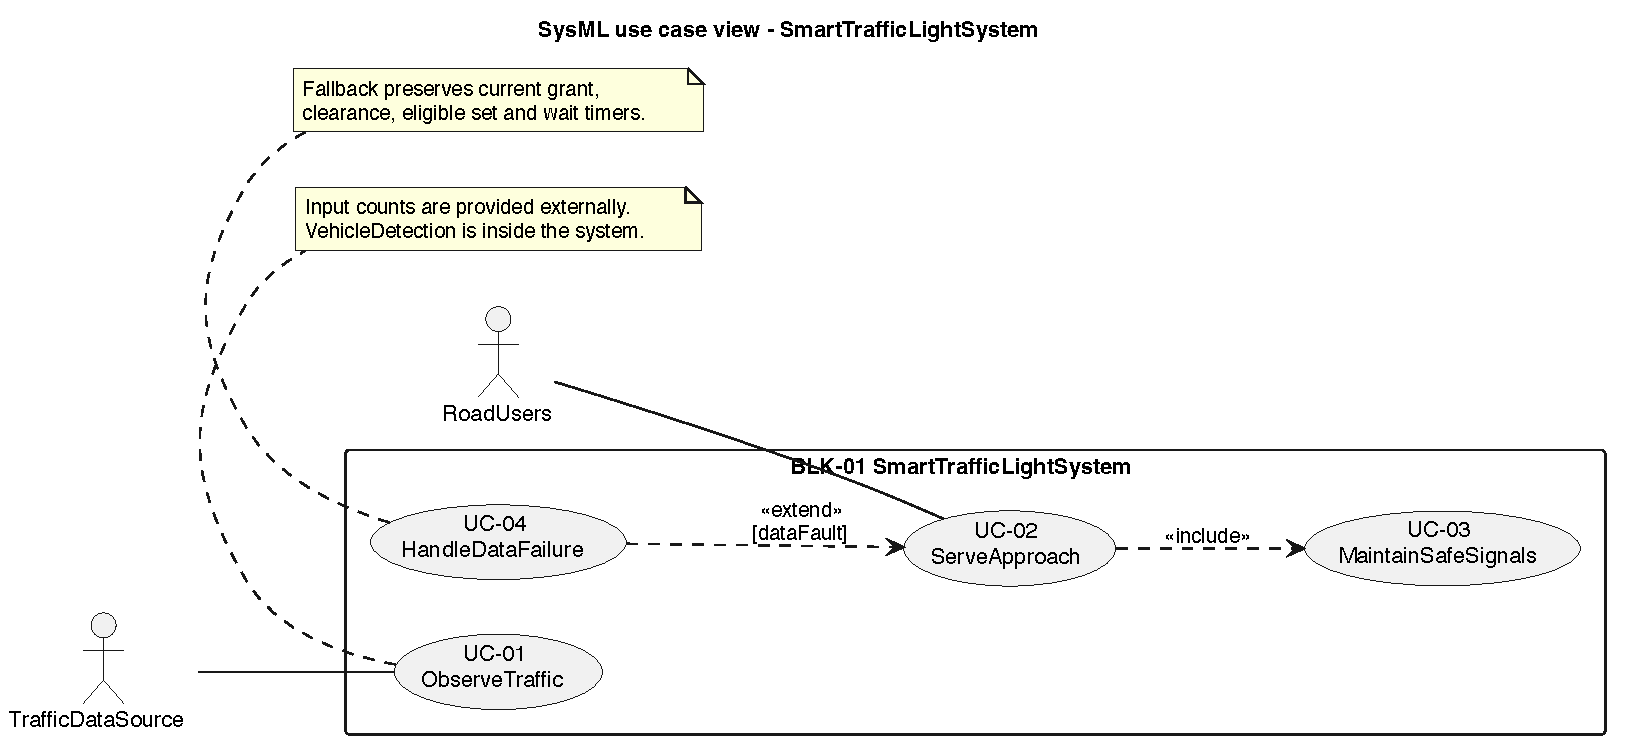
\includegraphics[width=.82\linewidth,height=.68\textheight,keepaspectratio]{use-case.pdf}
\vfill\scriptsize Sensor/adapter adalah komponen internal. UC-04 memperluas pelayanan saat dataFault; UC-03 diperlukan oleh UC-02.
\end{frame}

\begin{frame}{Behavior: grant tidak berubah di tengah green}
\begin{tabular}{lp{.64\linewidth}}\toprule State & Aturan baseline \\\midrule
Green(i) & Hanya i green; grant 10/20/30 s dibekukan \\[3mm]
Yellow(i) & Aktif 3 s setelah green berakhir \\[3mm]
Clearance & SemuaRed 1 s sebelum keputusan berikutnya \\[3mm]
Ready & Pilih eligible, cek deadline, validasi grant \\[3mm]
SafetyHold & SemuaRed hingga restart jika command/rencana tidak sah \\\bottomrule\end{tabular}
\vfill\small Ringkasan STM-01. DataFault sendiri tidak memotong green aktif.
\end{frame}

\begin{frame}{Structure: tanggung jawab dan flow}
\small
\begin{tabular}{p{.30\linewidth}p{.60\linewidth}}\toprule Block & Tanggung jawab / output \\\midrule
VehicleDetection & Validasi CountsFrame, status fault/recovery \\[2mm]
DensityAnalysis & Hitungan valid menjadi DensityFrame \\[2mm]
TrafficController & Eligibility, rank/deadline, PhaseCommand \\[2mm]
SignalController & Lifecycle/clearance, BoundaryEvent, LampVector \\[2mm]
TrafficLights[4] & Entry lampu sesuai approach masing-masing \\\bottomrule\end{tabular}
\vfill\small BDD mendefinisikan type; IBD memakai part dan port P01--P12. Connector bertipe dan terdokumentasi.
\end{frame}

\begin{frame}{Traceability: dari alasan ke pemeriksaan}
\begin{block}{Contoh requirement batas tunggu}
ASM-004/005/008 $\rightarrow$ REQ-P-005 $\rightarrow$ UC-02 / ACT-03 $\rightarrow$ TrafficController $\rightarrow$ VER-09
\end{block}
\vspace{4mm}
\begin{itemize}
\item Block $\xrightarrow{\text{satisfy}}$ requirement.
\item TestCase $\xrightarrow{\text{verify}}$ requirement.
\item Action $\xrightarrow{\text{allocate}}$ block.
\end{itemize}
\vfill\small Seluruh 24 requirement memiliki model dan verification link. Link tidak otomatis berarti test passed.
\end{frame}

\begin{frame}{Mengapa batas tunggu 210 s layak pada model?}
\begin{block}{Setiap pendekat dilayani sekali per round}
Kasus terburuk: pertama pada round r, terakhir pada round r+1.
\end{block}
\[W_{\max}\leq 6G_{\max}+7(Y+A)=6(30)+7(3+1)=208\text{ s}\]
\begin{itemize}
\item Checker:24$\times$24=576 pasangan urutan.
\item 2304 service waits diperiksa; maksimum 208 s.
\item Startup terburuk 103 s; batas desain 210 s.
\end{itemize}
\vfill\small Analisis kontrak round, bukan delay individual, antrean habis, atau throughput. Clock ideal; tidak mencakup SafetyHold/restart.
\end{frame}

\begin{frame}{Fault, fallback dan recovery}
\begin{columns}[T]
\column{.48\textwidth}
\begin{block}{Jika data invalid/stale}Latch fault. Selesaikan grant dan clearance; pada boundary berikutnya gunakan ring dengan green 10.\end{block}
\column{.48\textwidth}
\begin{block}{Untuk kembali Normal}Tiga frame lengkap baik dengan timestamp baru, lalu awal round berikutnya. Round/wait tidak direset.\end{block}
\end{columns}
\vspace{4mm}\textbf{Batas verifikasi:} timeline ini masih expected behavior; checker belum menjalankan phase engine/fault recovery lengkap.
\end{frame}

\begin{frame}{Kesimpulan dan batas hasil}
\begin{itemize}
\item Model:24 requirement, tujuh view dan 21 skenario.
\item Evidence jurnal, catatan kuliah, dan asumsi desain dipisahkan.
\item Analisis kategori/tie/input/output-state dan bound sudah dijalankan.
\item Belum mengukur throughput atau keselamatan hardware.
\end{itemize}
\vspace{3mm}\small Lanjutan: implementasi phase engine, uji fault/recovery, lalu kalibrasi perangkat/geometri bila scope diperluas. Peringatan xref PDF MBSE dan akses penerbit dicatat. Bantuan AI digunakan; kelompok tetap meninjau isi sebelum penyerahan.
\end{frame}

\begin{frame}{Referensi}
\tiny\bibliographystyle{plainnat}\bibliography{../report/bibliography}
\end{frame}
\end{document}
